\chapter{Teoría del campo de ligandos y color}\label{ch:b2:ligand-field}

El rubí es rojo y la esmeralda verde, y sin embargo ambos deben su color al mismo ion,
\ce{Cr^3+}, algunos de los cuales sustituyen al aluminio en el corindón, \ce{Al2O3}, o en el
berilo. Los cristales de sulfato de cobre son de un azul intenso, pero el polvo que queda tras
calentarlos es blanco. En cada caso el color procede de electrones que saltan
entre orbitales d cuyas energías han separado los átomos circundantes,
en una cantidad que depende de qué átomos rodean al ion y de cómo lo hacen. Este
capítulo calcula ese desdoblamiento, primero con cargas puntuales y luego con \omterm{def:b2:diatomic-mos:lcao}{orbitales
moleculares}; explica los colores, el magnetismo y la \omterm{def:b2:coordination-complexes:electron-count}{regla de los 18 electrones} del
capítulo anterior.

\begin{recall}
\Cref{ch:b2:coordination-complexes}: configuraciones $d^n$, geometrías, recuentos de
electrones. \Cref{ch:b2:atomic-orbitals}: las formas de los cinco orbitales d.
\Cref{ch:b2:fragment-orbitals}: \omterm{def:b2:fragment-orbitals:fragment}{orbitales de fragmento}. El volumen del primer año: absorbancia,
colores complementarios, electrones desapareados, regla de Hund.
\end{recall}

\begin{omfigure}
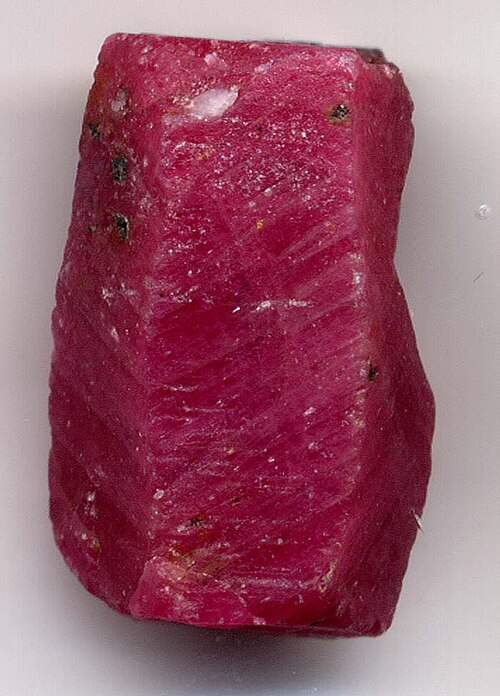
\includegraphics[height=3.6cm]{images/book3/ruby.jpg}\hspace{0.6cm}%
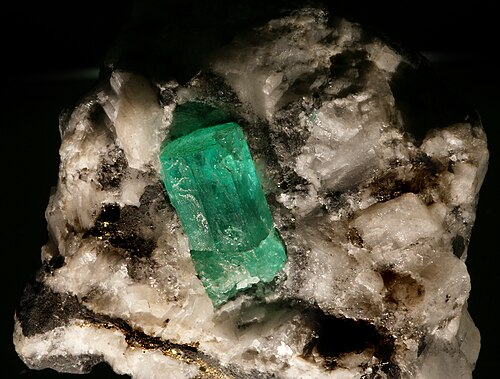
\includegraphics[height=3.6cm]{images/book3/emerald.jpg}\hspace{0.6cm}%
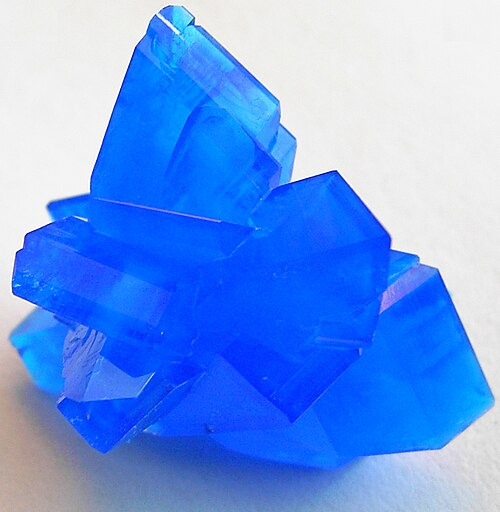
\includegraphics[height=3.6cm]{images/book3/copper-sulfate.jpg}

{\small Un cristal de rubí (dominio público); una esmeralda en su roca (Didier Descouens,
CC BY-SA 3.0); cristales de sulfato de cobre(II) pentahidratado (Stephanb, CC BY-SA
3.0). Wikimedia Commons. El cromo(III) da color a los dos primeros, y el acuocomplejo del
cobre(II), al tercero.}
\end{omfigure}

\section{El modelo del campo cristalino}

\begin{definition}[Campo cristalino]\label{def:b2:ligand-field:crystal-field}
El \emph{modelo del campo cristalino}\index{modelo del campo cristalino} trata los ligandos de un
complejo como cargas puntuales negativas (o extremos negativos de dipolos) alrededor del ion
metálico, y calcula cómo cambian las energías de sus orbitales d. En un campo
octaédrico, los orbitales d se desdoblan en dos conjuntos separados por el \emph{desdoblamiento del campo
cristalino}\index{desdoblamiento del campo cristalino} $\Delta_o$.
\end{definition}

Sitúense los seis ligandos sobre los ejes. Los orbitales $\mathrm d_{z^2}$ y $\mathrm d_{x^2-y^2}$
apuntan sus lóbulos directamente hacia los ligandos: un electrón en ellos sufre más repulsión
y suben. Los orbitales $\mathrm d_{xy}$, $\mathrm d_{xz}$, $\mathrm d_{yz}$ apuntan entre
los ligandos y suben menos. La primera pareja se llama $e_g$, y el segundo conjunto de tres,
$t_{2g}$ (nombres de la teoría de grupos, en el volumen del tercer año).

\begin{omfigure}
\begin{tikzpicture}[font=\small]
  \begin{scope}
    \pic at (0,0) {omdx2y2};
    \foreach \p in {(1.25,0),(-1.25,0),(0,1.25),(0,-1.25)} \node[circle, fill=black!70, inner sep=2.2pt] at \p {};
    \node at (0,-1.75) {$\mathrm d_{x^2-y^2}$: lóbulos hacia los ligandos};
  \end{scope}
  \begin{scope}[xshift=5.5cm]
    \pic at (0,0) {omdxy};
    \foreach \p in {(1.25,0),(-1.25,0),(0,1.25),(0,-1.25)} \node[circle, fill=black!70, inner sep=2.2pt] at \p {};
    \node at (0,-1.75) {$\mathrm d_{xy}$: lóbulos entre ellos};
  \end{scope}
\end{tikzpicture}

{\small Dos orbitales d entre los cuatro ligandos del plano $xy$ de un octaedro
(puntos negros). Los lóbulos de $\mathrm d_{x^2-y^2}$ apuntan hacia los ligandos, y los de
$\mathrm d_{xy}$, entre ellos.}
\end{omfigure}

\begin{theorem}[Baricentro]\label{thm:b2:ligand-field:barycentre}
En un campo octaédrico, medidas desde la energía media de los orbitales d, la
pareja $e_g$ está a $+0.6\Delta_o$ y el conjunto $t_{2g}$ a $-0.4\Delta_o$.
\end{theorem}

\begin{proof}
El campo eleva la media de las cinco energías d, pero el desdoblamiento no la cambia
(la regla del baricentro, admitida: la suma de los desplazamientos de un conjunto completo de
orbitales la fija la carga total, no su disposición). Con $e_g$ en $x$ y
$t_{2g}$ en $x - \Delta_o$, la condición $2x + 3(x - \Delta_o) = 0$ da $x = 0.6\Delta_o$.
\end{proof}

\section{Espín alto y espín bajo}

\begin{definition}[Estados de espín]\label{def:b2:ligand-field:spin}
La \emph{energía de apareamiento}\index{energia de apareamiento@energía de apareamiento} $P$ es la energía necesaria para poner un segundo
electrón en un orbital ocupado en lugar de en uno vacío de la misma energía. Un
complejo es de \emph{espín alto}\index{espin alto@espín alto} cuando sus electrones ocupan los orbitales $e_g$
antes de aparearse en $t_{2g}$, y de \emph{espín bajo}\index{espin bajo@espín bajo} cuando se aparean primero en $t_{2g}$.
\end{definition}

\begin{proposition}[Elección del estado de espín]\label{prop:b2:ligand-field:spin-state}
Para los iones octaédricos $d^4$ a $d^7$, el complejo es de \omterm{def:b2:ligand-field:spin}{espín bajo} si $\Delta_o > P$ y de \omterm{def:b2:ligand-field:spin}{espín alto}
si $\Delta_o < P$. Para $d^1$--$d^3$ y $d^8$--$d^{10}$ solo existe una configuración.
\end{proposition}

\begin{proof}
A partir de $d^3$ ($t_{2g}^3$), el cuarto electrón entra en $e_g$ (coste $\Delta_o$ por encima de
$t_{2g}$) o se aparea en $t_{2g}$ (coste $P$). Gana el más barato; la misma comparación vale
para cada electrón hasta $d^7$. Para $d^1$--$d^3$ hay sitio en $t_{2g}$ sin aparearse;
para $d^8$--$d^{10}$, $t_{2g}$ está lleno y hay que usar $e_g$ de todos modos.
\end{proof}

\begin{definition}[Energía de estabilización del campo cristalino]\label{def:b2:ligand-field:cfse}
La \emph{energía de estabilización del campo cristalino}\index{energia de estabilizacion del campo cristalino@energía de estabilización del campo cristalino}
(EECC) de una configuración $t_{2g}^ae_g^b$ es $(-0.4a + 0.6b)\Delta_o$, la energía de
los electrones d respecto del baricentro (contando aparte las \omterm{def:b2:ligand-field:spin}{energías de apareamiento}).
\end{definition}

\begin{proposition}[La EECC a lo largo de la serie]\label{prop:b2:ligand-field:cfse}
En \omterm{def:b2:ligand-field:spin}{espín alto}, la EECC vale $0$, $-0.4$, $-0.8$, $-1.2$, $-0.6$, $0$, $-0.4$, $-0.8$, $-1.2$,
$-0.6$, $0$ (en $\Delta_o$) para $d^0$ a $d^{10}$: se anula para $d^0$, $d^5$, $d^{10}$. En \omterm{def:b2:ligand-field:spin}{espín
bajo} alcanza $-2.4\Delta_o$ para $d^6$.
\end{proposition}

\begin{proof}
Se llenan las configuraciones y se aplica la definición; los valores son los de la figura,
calculados.
\end{proof}

\begin{omfigure}
\begin{tikzpicture}
\begin{axis}[width=0.55\linewidth, height=5cm, xmin=-0.5, xmax=10.5, ymin=-2.6, ymax=0.3,
  axis x line=bottom, axis y line=left, xlabel={$d^n$}, ylabel={EECC ($\Delta_o$)},
  xtick={0,1,2,3,4,5,6,7,8,9,10}, tick label style={font=\small}, label style={font=\small}]
\addplot[omThm, thick, mark=*, mark size=1.3pt] table[x=n, y=high] {figdata/out/bachelor-2-ligand-field-a.dat};
\addplot[omDef, thick, dashed, mark=square*, mark size=1.3pt] table[x=n, y=low] {figdata/out/bachelor-2-ligand-field-a.dat};
\node[font=\scriptsize, omThm, anchor=west] at (axis cs:5.4,0.0) {espín alto};
\node[font=\scriptsize, omDef, anchor=west] at (axis cs:6.6,-2.2) {espín bajo};
\end{axis}
\end{tikzpicture}\hfill
\begin{tikzpicture}[font=\small]
  \pic (t) at (0,0) {omlevel={ud}{0.5}}; \pic at (0.6,0) {omlevel={u}{0.5}}; \pic at (1.2,0) {omlevel={u}{0.5}};
  \pic at (0.3,1.6) {omlevel={u}{0.5}}; \pic at (0.9,1.6) {omlevel={u}{0.5}};
  \node at (0.6,-0.8) {$d^6$ de espín alto};
  \node[font=\scriptsize, anchor=east] at (-0.35,0) {$t_{2g}$}; \node[font=\scriptsize, anchor=east] at (-0.05,1.6) {$e_g$};
  \pic at (3,0) {omlevel={ud}{0.5}}; \pic at (3.6,0) {omlevel={ud}{0.5}}; \pic at (4.2,0) {omlevel={ud}{0.5}};
  \pic at (3.3,2.4) {omlevel={empty}{0.5}}; \pic at (3.9,2.4) {omlevel={empty}{0.5}};
  \node at (3.6,-0.8) {$d^6$ de espín bajo};
  \draw[<->, omProp] (4.7,0) -- (4.7,2.4) node[midway, right, font=\scriptsize] {$\Delta_o$};
  \draw[<->, omProp] (1.7,0) -- (1.7,1.6) node[midway, right, font=\scriptsize] {$\Delta_o$};
\end{tikzpicture}

{\small A la izquierda: \omterm{def:b2:ligand-field:cfse}{energía de estabilización del campo cristalino} a lo largo de la serie d (calculada),
en \omterm{def:b2:ligand-field:spin}{espín alto} (trazo continuo) y en \omterm{def:b2:ligand-field:spin}{espín bajo} (discontinuo). A la derecha: las dos configuraciones de un ion $d^6$:
cuatro electrones desapareados cuando $\Delta_o < P$ (como \ce{[Fe(H2O)6]^2+}), ninguno cuando $\Delta_o >
P$ (como \ce{[Fe(CN)6]^4-}).}
\end{omfigure}

\begin{method}[Estado de espín, EECC y electrones desapareados]\label{met:b2:ligand-field:spin-state}
\begin{enumerate}
  \item Hállese $n$ a partir del estado de oxidación ($n = g - m$).
  \item Para $d^4$--$d^7$, compárense $\Delta_o$ y $P$ (o sitúese el ligando en la
        \omterm{def:b2:ligand-field:spectrochemical}{serie espectroquímica}): campo fuerte, \omterm{def:b2:ligand-field:spin}{espín bajo}; campo débil, \omterm{def:b2:ligand-field:spin}{espín alto}.
  \item Llénense $t_{2g}$ y $e_g$ en consecuencia; EECC $= (-0.4a + 0.6b)\Delta_o$.
  \item Cuéntense los electrones desapareados; cualquier electrón desapareado hace
        \omterm{def:b2:diatomic-mos:magnetism}{paramagnético} el complejo.
\end{enumerate}
\end{method}

\section{Otras geometrías}

\begin{proposition}[Campos tetraédrico y plano-cuadrado]\label{prop:b2:ligand-field:tetrahedral}
En un campo tetraédrico el orden se invierte: dos orbitales ($e$) por debajo de tres ($t_2$),
con un desdoblamiento $\Delta_t \approx \frac49\Delta_o$ para el mismo metal y los mismos ligandos; los complejos
tetraédricos son de \omterm{def:b2:ligand-field:spin}{espín alto}. En un campo plano-cuadrado el orbital $\mathrm d_{x^2-y^2}$ está muy
por encima de los demás: un ion $d^8$ llena los cuatro orbitales inferiores y lo deja vacío.
\end{proposition}

\admitted

El factor $4/9$ procede de la geometría de las cargas puntuales; con solo cuatro ligandos,
ninguno de ellos sobre los ejes, el desdoblamiento es demasiado pequeño para superar la \omterm{def:b2:ligand-field:spin}{energía
de apareamiento}. Retirar los dos ligandos del eje $z$ de un octaedro rebaja los orbitales con
componente $z$ y no eleva ninguno: esto explica los complejos $d^8$ plano-cuadrados del
capítulo anterior, cuyos ocho electrones encuentran todos sitio por debajo del
$\mathrm d_{x^2-y^2}$ vacío.

\begin{omfigure}
\begin{tikzpicture}[font=\scriptsize]
  % octahedral
  \pic at (-0.3,0) {omlevel={empty}{0.45}}; \pic at (0.25,0) {omlevel={empty}{0.45}}; \pic at (0.8,0) {omlevel={empty}{0.45}};
  \pic at (0,1.8) {omlevel={empty}{0.45}}; \pic at (0.55,1.8) {omlevel={empty}{0.45}};
  \node[anchor=west] at (1.1,0) {$t_{2g}$}; \node[anchor=west] at (0.85,1.8) {$e_g$};
  \node[font=\small] at (0.25,-0.7) {octaédrico};
  % tetrahedral
  \begin{scope}[xshift=3.5cm]
    \pic at (0,0.6) {omlevel={empty}{0.45}}; \pic at (0.55,0.6) {omlevel={empty}{0.45}};
    \pic at (-0.3,1.4) {omlevel={empty}{0.45}}; \pic at (0.25,1.4) {omlevel={empty}{0.45}}; \pic at (0.8,1.4) {omlevel={empty}{0.45}};
    \node[anchor=west] at (0.85,0.6) {$e$}; \node[anchor=west] at (1.1,1.4) {$t_2$};
    \node[font=\small] at (0.25,-0.7) {tetraédrico};
  \end{scope}
  % square planar
  \begin{scope}[xshift=7cm]
    \pic at (0,-0.2) {omlevel={empty}{0.45}}; \pic at (0.55,-0.2) {omlevel={empty}{0.45}};
    \pic at (0.25,0.3) {omlevel={empty}{0.45}};
    \pic at (0.25,0.9) {omlevel={empty}{0.45}};
    \pic at (0.25,2.6) {omlevel={empty}{0.45}};
    \node[anchor=west] at (0.85,-0.2) {$\mathrm d_{xz}, \mathrm d_{yz}$};
    \node[anchor=west] at (0.55,0.3) {$\mathrm d_{z^2}$};
    \node[anchor=west] at (0.55,0.9) {$\mathrm d_{xy}$};
    \node[anchor=west] at (0.55,2.6) {$\mathrm d_{x^2-y^2}$};
    \node[font=\small] at (0.25,-0.7) {plano-cuadrado};
  \end{scope}
\end{tikzpicture}

{\small Desdoblamiento de los orbitales d en tres geometrías, esquema (no a la misma
escala): octaédrica, tetraédrica (invertida y menor) y plano-cuadrada (un orbital muy
por encima de los demás).}
\end{omfigure}

\section{El color y la serie espectroquímica}

\begin{definition}[Transición d--d]\label{def:b2:ligand-field:d-d}
Una \emph{transición d--d}\index{transicion d--d@transición d--d} es la promoción de un electrón de un
nivel d inferior a otro superior de un complejo por absorción de luz; para un ion $d^1$, de
$t_{2g}$ a $e_g$, con la energía $\Delta_o$.
\end{definition}

\begin{proposition}[El desdoblamiento a partir del color]\label{prop:b2:ligand-field:colour}
Si un complejo absorbe con máxima intensidad a la longitud de onda $\lambda_{\max}$ por una \omterm{def:b2:ligand-field:d-d}{transición d--d}
de energía $\Delta_o$, entonces $\Delta_o = N_Ahc/\lambda_{\max}$ por mol, o $\tilde\nu = 1/\lambda_{\max}$
en números de onda; el color que se ve es el complementario del color absorbido.
\end{proposition}

\begin{proof}
Un fotón de longitud de onda $\lambda$ lleva $hc/\lambda$; un mol de fotones, $N_Ahc/\lambda$. La luz
blanca menos la banda absorbida se ve del color complementario.
\end{proof}

\begin{method}[De una banda de absorción a un color]\label{met:b2:ligand-field:colour}
\begin{enumerate}
  \item Conviértase $\lambda_{\max}$ en $\tilde\nu = 1/\lambda_{\max}$ (\unit{cm^{-1}}) y en
        $N_Ahc/\lambda_{\max}$ (\unit{kJ/mol}): $\qty{500}{nm} \leftrightarrow \qty{20000}{cm^{-1}}
        \leftrightarrow \qty{239}{kJ/mol}$.
  \item Hállese el color absorbido (violeta 400--430, azul 430--490, verde 490--560, amarillo
        560--590, naranja 590--620, rojo 620--700 nm, aproximadamente).
  \item El color que se ve está en el lado opuesto de la rueda de colores.
\end{enumerate}
\end{method}

\begin{omfigure}
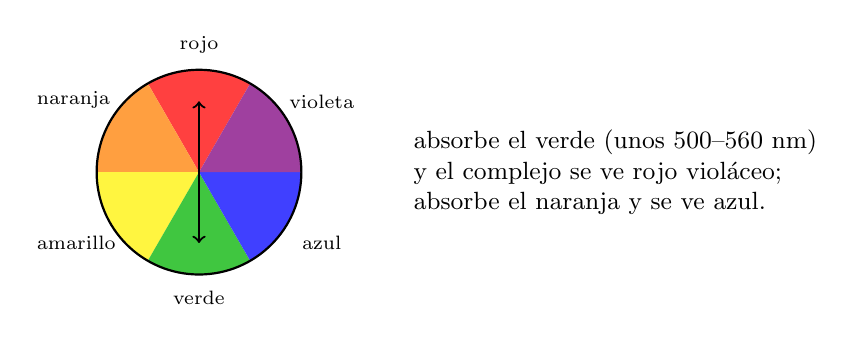
\begin{tikzpicture}[font=\scriptsize]
  \foreach \a/\c/\n in {90/red/rojo, 150/orange/naranja, 210/yellow/amarillo, 270/green!70!black/verde, 330/blue/azul, 30/violet/violeta} {
    \fill[\c!75] (0,0) -- (\a-30:1.3) arc[start angle=\a-30, end angle=\a+30, radius=1.3] -- cycle;
    \node[anchor=\a+180] at (\a:1.38) {\n};
  }
  \draw[thick] (0,0) circle (1.3);
  \draw[<->, thick] (90:0.9) -- (270:0.9);
  \node[anchor=west, font=\small, align=left] at (2.6,0) {absorbe el verde (unos 500--560 nm)\\ y el complejo se ve rojo violáceo;\\ absorbe el naranja y se ve azul.};
\end{tikzpicture}

{\small Una rueda de colores: el color que se ve es aproximadamente el complementario, diametralmente
opuesto, de la banda absorbida.}
\end{omfigure}

\begin{definition}[Serie espectroquímica]\label{def:b2:ligand-field:spectrochemical}
La \emph{serie espectroquímica}\index{serie espectroquimica@serie espectroquímica} ordena los ligandos según el
desdoblamiento que producen para un ion metálico dado:
\[
  \ce{I-} < \ce{Br-} < \ce{Cl-} < \ce{F-} < \ce{OH-} < \ce{H2O} < \ce{NH3} < \text{en} <
  \ce{NO2-} < \ce{CN-} < \ce{CO} .
\]
Para un ligando dado, $\Delta_o$ también crece con la carga del ion metálico y al bajar en un grupo
(los complejos 4d y 5d, más grandes que los 3d, son casi siempre de \omterm{def:b2:ligand-field:spin}{espín bajo}).
\end{definition}

Los haluros están en el extremo débil, y \ce{CN-} y \ce{CO} en el fuerte, lo que el
\omterm{def:b2:ligand-field:crystal-field}{modelo del campo cristalino} no puede explicar: pondría el \ce{F-}, cargado, por encima del \ce{CO},
neutro. La explicación necesita orbitales.

\section{El campo de ligandos}

\begin{definition}[Teoría del campo de ligandos]\label{def:b2:ligand-field:ligand-field}
La \emph{teoría del campo de ligandos}\index{teoria del campo de ligandos@teoría del campo de ligandos} describe un complejo con \omterm{def:b2:diatomic-mos:lcao}{orbitales moleculares}
construidos a partir de los orbitales de valencia del metal (sus nueve orbitales $n$d, $(n+1)$s y $(n+1)$p)
y los orbitales dadores de los ligandos.
\end{definition}

\begin{proposition}[Enlace $\sigma$ en un complejo octaédrico]\label{prop:b2:ligand-field:mo-octahedral}
Con seis ligandos que aportan cada uno un orbital dador $\sigma$, se forman seis \omterm{def:b2:diatomic-mos:lcao}{orbitales moleculares} enlazantes
a partir del s, los tres p y los dos orbitales d $e_g$ del metal; los tres orbitales $t_{2g}$, que
apuntan entre los ligandos, permanecen no enlazantes; por encima de ellos están los \omterm{def:b2:diatomic-mos:bonding}{orbitales antienlazantes}
$e_g^*$. Los electrones de los ligandos llenan los seis \omterm{def:b2:diatomic-mos:bonding}{orbitales enlazantes}; los electrones d del metal van
a $t_{2g}$ y $e_g^*$, separados por $\Delta_o$. Los \omterm{def:b2:diatomic-mos:bonding}{orbitales enlazantes} y no enlazantes pueden contener
$12 + 6 = 18$ electrones.
\end{proposition}

\begin{proof}[Argumento]
Por el método de los fragmentos del \cref{ch:b2:fragment-orbitals}, cada orbital del metal interacciona
con la combinación de orbitales de los ligandos de la misma simetría: el s con la totalmente
simétrica, cada p con una pareja de ligandos opuestos, $\mathrm d_{z^2}$ y $\mathrm
d_{x^2-y^2}$ con las combinaciones que apuntan según sus lóbulos; ninguna combinación $\sigma$
corresponde a los orbitales $t_{2g}$ (su solapamiento con cualquier dador $\sigma$ que apunte a lo largo de un eje
es nulo por simetría). Los nombres de las combinaciones proceden de la teoría de grupos, que se admite.
Llenar todos los \omterm{def:b2:diatomic-mos:bonding}{orbitales enlazantes} y no enlazantes, y ninguno de los antienlazantes, requiere
18 electrones: la \omterm{def:b2:coordination-complexes:electron-count}{regla de los 18 electrones}.
\end{proof}

\begin{omfigure}
\begin{tikzpicture}[font=\scriptsize]
  % metal
  \pic (m4p1) at (-0.45,2.6) {omlevel={empty}{0.4}}; \pic (m4p2) at (0,2.6) {omlevel={empty}{0.4}}; \pic (m4p3) at (0.45,2.6) {omlevel={empty}{0.4}};
  \node[anchor=east] at (-0.7,2.6) {$(n{+}1)$p};
  \pic (m4s) at (0,1.8) {omlevel={empty}{0.6}}; \node[anchor=east] at (-0.35,1.8) {$(n{+}1)$s};
  \foreach \x in {-0.9,-0.45,0,0.45,0.9} \pic at (\x,0.6) {omlevel={empty}{0.4}};
  \coordinate (m3d) at (1.1,0.6); \node[anchor=east] at (-1.15,0.6) {$n$d};
  \node[font=\small] at (0,-2.9) {metal};
  % ligands
  \foreach \x in {6.2,6.72,7.24,7.76,8.28,8.8} \pic at (\x,-0.9) {omlevel={ud}{0.36}};
  \coordinate (lig) at (6.0,-0.9);
  \node[font=\small] at (7.3,-2.9) {seis orbitales dadores $\sigma$};
  % MOs
  \pic (b1) at (3.6,-2.4) {omlevel={ud}{0.5}};
  \foreach \x in {3.0,3.6,4.2} \pic at (\x,-1.9) {omlevel={ud}{0.5}};
  \pic at (3.3,-1.45) {omlevel={ud}{0.5}}; \pic at (3.9,-1.45) {omlevel={ud}{0.5}};
  \foreach \x in {3.0,3.6,4.2} \pic at (\x,0.3) {omlevel={empty}{0.5}};
  \pic at (3.3,1.5) {omlevel={empty}{0.5}}; \pic at (3.9,1.5) {omlevel={empty}{0.5}};
  \pic at (3.6,3.1) {omlevel={empty}{0.5}};
  \foreach \x in {3.0,3.6,4.2} \pic at (\x,3.6) {omlevel={empty}{0.5}};
  \node[anchor=north] at (3.6,0.12) {$t_{2g}$ (no enlazantes)};
  \node[anchor=west] at (4.2,1.5) {$e_g^*$};
  \node[anchor=north] at (3.6,-2.58) {6 enlazantes};
  \draw[<->, omProp] (2.55,0.3) -- (2.55,1.5) node[midway, right] {$\Delta_o$};
  \draw[omcorr, densely dashed] (m3d) -- (2.75,0.3) (m3d) -- (3.05,1.5) (1.1,0.6) -- (3.05,-1.45);
  \draw[omcorr, densely dashed] (lig) -- (4.15,-1.45) (lig) -- (4.45,-1.9) (lig) -- (3.85,-2.4) (lig) -- (4.15,1.5);
  \draw[omcorr, densely dashed] (m4s-r) -- (3.35,-2.4) (m4s-r) -- (3.35,3.1) (m4p3-r) -- (2.75,-1.9) (m4p3-r) -- (2.75,3.6);
\end{tikzpicture}

{\small \omterm{def:b2:diatomic-mos:lcao}{Orbitales moleculares} de un complejo octaédrico con seis dadores $\sigma$,
esquema. Los doce electrones de los ligandos llenan los seis \omterm{def:b2:diatomic-mos:bonding}{orbitales enlazantes}; los electrones d
del metal ocupan los niveles $t_{2g}$, no enlazantes, y $e_g^*$, antienlazantes, separados por
$\Delta_o$: se recupera la imagen del campo cristalino. Hasta 18 electrones llenan los niveles
enlazantes y no enlazantes.}
\end{omfigure}

\begin{definition}[Ligandos $\pi$-dadores y $\pi$-aceptores]\label{def:b2:ligand-field:pi-ligands}
Un \emph{ligando $\pi$-dador}\index{ligando pi-dador@ligando $\pi$-dador} tiene orbitales llenos
de simetría $\pi$ respecto del enlace metal--ligando (pares no enlazantes de \ce{Cl-},
\ce{OH-}); un \emph{ligando $\pi$-aceptor}\index{ligando pi-aceptor@ligando $\pi$-aceptor}
los tiene vacíos y de baja energía (los orbitales $\pi^*$ de \ce{CO} y de \ce{CN-}). La transferencia de
densidad electrónica de los orbitales d llenos del metal a los orbitales $\pi^*$ vacíos de un
ligando $\pi$-aceptor se llama \emph{retrodonación}\index{retrodonacion@retrodonación}.
\end{definition}

\begin{proposition}[Efectos $\pi$ sobre el desdoblamiento]\label{prop:b2:ligand-field:pi-effects}
Los ligandos $\pi$-dadores reducen $\Delta_o$; los ligandos $\pi$-aceptores lo aumentan.
\end{proposition}

\begin{proof}
Los orbitales $t_{2g}$ tienen la simetría adecuada para solaparse con los orbitales $\pi$ de los ligandos. Un orbital
$\pi$ lleno del ligando está por debajo de $t_{2g}$: por el \cref{thm:b2:frontier-orbitals:perturbation}, la
interacción empuja $t_{2g}$ hacia arriba, hacia $e_g^*$, y $\Delta_o$ disminuye. Un orbital $\pi^*$ vacío
está por encima de $t_{2g}$: la interacción empuja $t_{2g}$ hacia abajo, y $\Delta_o$ aumenta. El segundo caso
transfiere densidad d del metal al $\pi^*$ del ligando: es la \omterm{def:b2:ligand-field:pi-ligands}{retrodonación}.
\end{proof}

\begin{omfigure}
\begin{tikzpicture}[font=\scriptsize]
  \begin{scope}
    \pic (t) at (0,1.2) {omlevel={empty}{0.6}}; \node[anchor=east] at (-0.35,1.2) {$t_{2g}$};
    \pic (l) at (2.4,0) {omlevel={ud}{0.6}}; \node[anchor=west] at (2.75,0) {$\pi$ del ligando (lleno)};
    \pic (n) at (1.2,1.75) {omlevel={empty}{0.6}};
    \draw[omcorr, densely dashed] (t-r) -- (n-l) (l-l) -- (n-r);
    \pic (e) at (1.2,3.0) {omlevel={empty}{0.6}}; \node[anchor=west] at (1.55,3.0) {$e_g^*$};
    \draw[<->, omProp] (0.55,1.75) -- (0.55,3.0) node[midway, left] {$\Delta_o$ menor};
    \node[font=\small] at (1.2,-0.8) {dador $\pi$};
  \end{scope}
  \begin{scope}[xshift=6.5cm]
    \pic (t) at (0,1.2) {omlevel={empty}{0.6}}; \node[anchor=east] at (-0.35,1.2) {$t_{2g}$};
    \pic (l) at (2.4,2.6) {omlevel={empty}{0.6}}; \node[anchor=west] at (2.75,2.6) {$\pi^*$ del ligando (vacío)};
    \pic (n) at (1.2,0.65) {omlevel={empty}{0.6}};
    \draw[omcorr, densely dashed] (t-r) -- (n-l) (l-l) -- (n-r);
    \pic (e) at (1.2,3.0) {omlevel={empty}{0.6}}; \node[anchor=west] at (1.55,3.15) {$e_g^*$};
    \draw[<->, omProp] (0.55,0.65) -- (0.55,3.0) node[midway, left] {$\Delta_o$ mayor};
    \node[font=\small] at (1.2,-0.8) {aceptor $\pi$ (retrodonación)};
  \end{scope}
\end{tikzpicture}

{\small Efecto de los orbitales $\pi$ de los ligandos sobre el nivel $t_{2g}$, esquema. Un orbital $\pi$
lleno del ligando, situado por debajo, empuja $t_{2g}$ hacia arriba (menor desdoblamiento); un orbital $\pi^*$ vacío situado por encima lo
empuja hacia abajo (mayor desdoblamiento).}
\end{omfigure}

Esto sitúa \ce{CO} y \ce{CN-}, fuertes dadores $\sigma$ y aceptores $\pi$, en lo alto de la
\omterm{def:b2:ligand-field:spectrochemical}{serie espectroquímica}, y los haluros, dadores $\pi$, en lo más bajo. Los carbonilos metálicos tienen
sus orbitales $t_{2g}$ estabilizados y llenos: los complejos de 18 electrones del
\cref{ch:b2:coordination-complexes}.

\section{Ejercicios}

\begin{exercise}[$\star$]\label{exo:b2:ligand-field:1}
Dense la configuración octaédrica y la EECC de un ion $d^3$ y de un ion $d^8$.
\end{exercise}

\begin{exercise}[$\star$]\label{exo:b2:ligand-field:2}
¿Cuántos electrones desapareados tienen \ce{[Fe(H2O)6]^2+} (de \omterm{def:b2:ligand-field:spin}{espín alto}) y \ce{[Fe(CN)6]^4-} (de \omterm{def:b2:ligand-field:spin}{espín
bajo})?
\end{exercise}

\begin{exercise}[$\star$]\label{exo:b2:ligand-field:3}
Un complejo absorbe con máxima intensidad a \qty{600}{nm}. ¿De qué color se ve?
\end{exercise}

\begin{exercise}[$\star$]\label{exo:b2:ligand-field:4}
Ordénense \ce{H2O}, \ce{CN-}, \ce{Cl-}, \ce{NH3} según el desdoblamiento que producen.
\end{exercise}

\begin{exercise}[$\star\star$]\label{exo:b2:ligand-field:5}
Para un ion $d^5$, $\Delta_o = \qty{165}{kJ/mol}$ con el agua y $\qty{390}{kJ/mol}$ con el cianuro,
y $P = \qty{300}{kJ/mol}$ (datos del ejercicio). Prevéanse ambos estados de espín y los electrones
desapareados.
\end{exercise}

\begin{exercise}[$\star\star$]\label{exo:b2:ligand-field:6}
\ce{[Co(H2O)6]^2+} es rosa, y \ce{[CoCl4]^2-}, azul intenso. Explíquese el cambio de color a partir del
cambio de geometría y de ligando.
\end{exercise}

\begin{exercise}[$\star\star$]\label{exo:b2:ligand-field:7}
Demuéstrese que el \ce{[Ni(CN)4]^2-} plano-cuadrado es \omterm{def:b2:diatomic-mos:magnetism}{diamagnético}, mientras que el
\ce{[NiCl4]^2-} tetraédrico tiene dos electrones desapareados.
\end{exercise}

\begin{exercise}[$\star\star$]\label{exo:b2:ligand-field:8}
Un complejo $d^1$ absorbe a \qty{500}{nm} (datos del ejercicio). Calcúlese $\Delta_o$ en \unit{cm^{-1}} y en
\unit{kJ/mol}.
\end{exercise}

\begin{exercise}[$\star\star$]\label{exo:b2:ligand-field:9}
¿Por qué son incoloros los compuestos de \ce{Zn^2+} y de \ce{Sc^3+}?
\end{exercise}

\begin{exercise}[$\star\star\star$]\label{exo:b2:ligand-field:10}
Cuéntense los electrones en los \omterm{def:b2:diatomic-mos:lcao}{orbitales moleculares} de \ce{[Co(NH3)6]^3+}: ¿qué niveles están llenos,
y es \omterm{def:b2:diatomic-mos:magnetism}{diamagnético} el complejo?
\end{exercise}

\begin{exercise}[$\star\star\star$]\label{exo:b2:ligand-field:11}
Explíquese por qué \ce{CO}, una molécula neutra y poco básica, produce un desdoblamiento mayor que
el ion fluoruro.
\end{exercise}

\begin{exercise}[$\star\star\star$]\label{exo:b2:ligand-field:12}
Las entalpías de hidratación de los iones \ce{M^2+} de \ce{Ca^2+} a \ce{Zn^2+}, representadas frente a $n$, forman
dos jorobas por encima de una recta que pasa por $d^0$, $d^5$ y $d^{10}$. Explíquese la forma con la
EECC de \omterm{def:b2:ligand-field:spin}{espín alto}.
\end{exercise}

\section{Problema: el rubí rojo y la esmeralda verde}

\begin{problem}[{Problema de fin de semana --- el cromo(III) en un campo octaédrico, las bandas de absorción
del rubí y el color que dejan, el campo más débil de la esmeralda, y el sulfato de cobre hidratado y
anhidro}]
\label{pb:b2:ligand-field:1}
Datos fijados para el problema (redondeados, ilustrativos): el rubí (\ce{Cr^3+} en \ce{Al2O3}) absorbe
en dos bandas, hacia \qty{556}{nm} y \qty{405}{nm}; en la esmeralda (\ce{Cr^3+} en el berilo) la
primera banda está hacia \qty{620}{nm}. Para un ion $d^3$ la primera banda corresponde a
$\Delta_o$. $N_Ahc = \qty{0.1196}{J.m/mol}$.
% ledger: const:NA, const:h, const:c

\medskip
\noindent\textbf{Parte I --- El cromo(III).}
\begin{enumerate}
  \item Dese la configuración $d^n$ de \ce{Cr^3+}.
  \item ¿Cómo se reparte en un campo octaédrico?
  \item ¿Hay elección entre \omterm{def:b2:ligand-field:spin}{espín alto} y \omterm{def:b2:ligand-field:spin}{espín bajo}?
  \item Calcúlese su EECC.
  \item ¿Cuántos electrones desapareados tiene?
  \item ¿Por qué los complejos de cromo(III) son cinéticamente inertes (lentos para intercambiar ligandos)?
\end{enumerate}

\medskip
\noindent\textbf{Parte II --- El rubí.}
\begin{enumerate}[resume]
  \item ¿Qué rodea a un ion \ce{Cr^3+} que sustituye a \ce{Al^3+} en el corindón?
  \item Conviértase la primera banda en número de onda.
  \item Dedúzcase $\Delta_o$ en \unit{kJ/mol}.
  \item ¿Qué colores absorben las dos bandas?
  \item ¿Qué queda para ver?
  \item ¿Por qué hay dos bandas para un solo desdoblamiento? (Basta una respuesta cualitativa.)
\end{enumerate}

\medskip
\noindent\textbf{Parte III --- La esmeralda.}
\begin{enumerate}[resume]
  \item Conviértase la banda de la esmeralda en $\Delta_o$.
  \item Compárese con el rubí: ¿qué cristal da el campo más fuerte?
  \item ¿Hacia dónde se desplaza el color absorbido, y qué color se transmite?
  \item Propóngase una razón estructural para el campo más débil del berilo.
  \item ¿Cambiaría el número de electrones desapareados?
\end{enumerate}

\medskip
\noindent\textbf{Parte IV --- El sulfato de cobre.}
\begin{enumerate}[resume]
  \item ¿Cuál es la configuración de \ce{Cu^2+}?
  \item En \ce{CuSO4.5H2O}, el cobre está rodeado de moléculas de agua. ¿Por qué es azul el sólido?
  \item ¿Qué le ocurre al color cuando se elimina el agua, y por qué?
  \item ¿Por qué una gota de agua vuelve a poner azul el polvo blanco?
  \item ¿Absorbería \ce{[Cu(NH3)4]^2+} a una longitud de onda más corta o más larga que el acuocomplejo?
  \item ¿Puede un ion $d^9$ ser de \omterm{def:b2:ligand-field:spin}{espín alto} o de \omterm{def:b2:ligand-field:spin}{espín bajo}?
  \item ¿Es \omterm{def:b2:diatomic-mos:magnetism}{paramagnético} \ce{CuSO4.5H2O}?
  \item Indíquese el $\Delta_o$ de \ce{Cr^3+} en el rubí a partir de su primera banda de absorción.
\end{enumerate}
\end{problem}
